\chapter{绪论}\label{ch:introduction}

\section{课题研究背景}\label{sec:research_background}
% Task-Oriented and Chat-Oriented.
早期的对话系统的主要用途是帮助用户用自然语言完成某项任务,
比如技术支持(Technical Support),预订机票、预订餐馆的座位、查询航班等。
这类系统又被称为面向任务的系统(Task-Oriented Dialogue System),
它们的实现技术包括关键词匹配、规则和模板以及对话状态追踪
(Dialogue State Tracking)等等,
往往需要大量人工标注的数据。
这些系统只能处理特定领域内的对话,不能回答开放性问题,用途局限于特定领域
\upcite{corpus_survey,Seq2Seq,Shang}。

随着在线聊天的流行,社交媒体和互联网论坛积累了大量的聊天语料数据,
具有代表性的社交媒体和论坛有Twitter,Reddit和微博。
大量的数据使人们可以构建数据驱动的(Data-Driven),
开放领域(Open-Domain)的对话系统\upcite{Ritter11},
这类对话系统又称为面向闲聊的系统(Chat-Oriented Dialogue System)。
这种系统能根据对话的上下文和用户的提问产生语义相关的回答,
用途有娱乐、语言学习工具和陪伴\upcite{HRED}等等。

开放领域的对话系统主要考察二人对话,
两人聊天的历史记录称为上下文(Context),记为$c$;
当前说话的人说出的话语称为消息(Message),记为$m$;
另外一个人对该消息的回复称为响应(Response),记为$r$。
$c,m,r$三者的关系如图~\ref{fig:context_message_response}~所示。
系统的输入是$c, m$,输出是$r$,
也就是输入对话的上下文和消息,输出响应,
这个问题被称为对话响应生成(Dialogue Response Generation)。

\begin{figure}[H]
    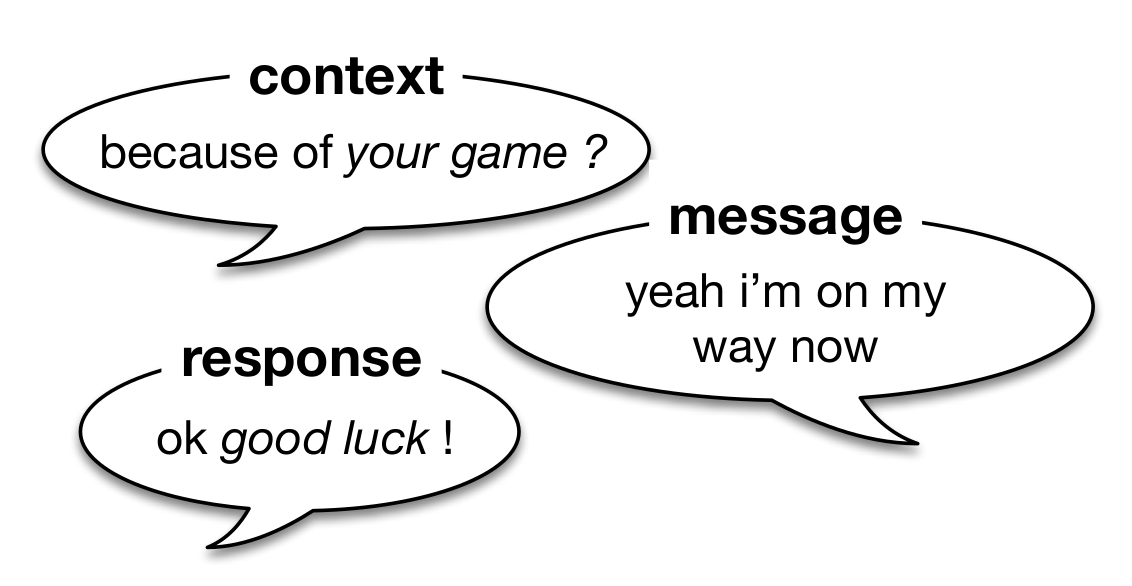
\includegraphics[width=0.6\textwidth]{figure/context_message_response.png}
    \centering
    \caption{上下文,消息和响应的关系\upcite{DCGM}}
    \label{fig:context_message_response}
\end{figure}

% Retrieval and Generative.
对话系统又可以分为生成式对话系统(Generative System)和检索式对话系统(Retrieval-based System)
\upcite{corpus_survey,NUC}。
简单来说,如果一个系统能生成训练集里没有出现过的句子,
就把它称为生成式系统\upcite{HowNot},反之称为检索式系统。
生成式系统建立了给定输入句子,所有输出句子的条件概率分布,并从这个分布中生成句子。
在解码(Decode)时,
由于可能的句子空间过于庞大,在实际中通常采用某种启发式搜索方法,
如集束搜索(Beam Search),贪婪搜索(Greedy Search)
和随机取样(Random Sample)等等,产生一个次优解。
设$X$为输入句子,$Y$为输出句子,$U$是全部句子的集合,生成式模型的一般表示为:
\begin{align}
    Y = \argmax_{Y\in U} p(Y|X)
\end{align}
实际中$\argmax$会被某种搜索算法代替。

检索式系统根据输入句子从一个文库$C$中检索输出句子。
$C$通常由人类撰写的语句组成,并且足够大,使得输出句子不容易重复。
系统通过某种打分机制,如词频-逆文档频率(Term Frequency-Inverse Document Frequency,TF-IDF)或语义相似度(Semantic Similarity),
对数据库中的候选句子进行打分,并把得分较高的候选句子作为输出:
\begin{align}
    Y = \argmax_{Y\in C} \textit{Score}(Y, X)
\end{align}

可见,生成式系统和检索式系统的根本区别在于获得输出句子的机制不同。
这两种方法各有优劣:检索式模型的输出没有语法错误并且可以筛选输出的内容\upcite{NUC},但是不能生成新句子;
生成式的模型能端对端的训练而且可以生成新的句子\upcite{Shang},但是容易生成过短的句子\upcite{AdverEval}。
在实际环境中,通常将它们作为模型联合体(Model Ensemble)使用\upcite{Two_are_better_than_one},
而检索式系统也经常作为生成式系统的基线系统\upcite{Shang,DCGM}。

% RNN, Seq2Seq and Embedding
生成式模型的流行得益于自然语言处理领域发展的一系列基础技术,包括
为单词提供平滑特征的词嵌入(Word Embedding)\upcite{NNLM,word2vec,Glove};
能对变长序列建模的循环神经网络语言模型(Recurrent Neural Networks Language Model,RNNLM)\upcite{RNNLM};
易于训练,能避免梯度消失问题\upcite{VanishingGradient}的循环门单元,如长短期记忆单元(Long Short-Term Memory,LSTM)
\upcite{LSTM}和门循环单元(Gated Recurrent Unit,GRU)\upcite{GRU};
以及序列到序列框架(Sequence to Sequence Framework,Seq2Seq)\upcite{Seq2Seq,GRU}。

% Chatbot in Seq2Seq.
Seq2Seq框架在自然语言处理的多项任务上都超过了之前的最佳水平,因此被广泛应用到对话生成领域。
在国外,最早把Seq2Seq用到对话生成领域的是Vinyals等人\upcite{GoogleChatbot},
他们在OpenSubtitles\upcite{opensub}
上训练的模型能回答简单的常识问题,
并且比基于规则的系统CleverBot\footnote{http://www.cleverbot.com/}获得了更高的人类评价得分。

% -- Li -- %
Li等人提出了一系列基于Seq2Seq框架的对话系统,包括
利用最大互信息(Maximum Mutual Information,MMI)增加输出多样性的目标函数\upcite{MMI};
在解码器端(Decoder)加入说话人身份信息(Speaker ID),促进输出的人格一致性(Personality Coherence)
\upcite{persona};
利用对抗生成网络(Generative Adversarial Networks,GAN)
\upcite{GAN}使系统输出和人类输出难以分辨\upcite{Adversarial} 等等。

% -- Serban -- %
Serban等人把Sordoni等人提出的用于查询建议(Query Suggestion)的
多层编解码器(Hierarchical Recurrent Encoder-Decoder,HRED)\upcite{hred-qs}应用到对话生成领域,
提出了能捕捉对话的层级结构的HRED模型\upcite{HRED}。
基于HRED,Serban等人又提出了利用随机潜变量(Stochastic Latent Variable)增加对话多样性的Variational Hierarchical Recurrent Encoder-Decoder,即VHRED\upcite{VHRED};
以及加入了高层次抽象信息的多精度循环网络(Multiresolution Recurrent Neural Networks,MultiRNN)\upcite{MrRNN}。

% -- Shang -- %
在国内,Shang等人研究了微博数据集上的短文本对话生成问题(Short-Text Conversation),
提出了以GRU为门单元的编解码器模型(Neural Response Machine,NRM)\upcite{Shang},
并在人类评价上取得了比检索式系统和翻译式系统\upcite{Ritter11}更好的成绩。
Chen Xing等人加入了从预训练LDA模型中获取的主题词(Topic Words),提出了Topic-Aware Seq2Seq \upcite{Topic_Aware},
由于篇幅有限,不能一一介绍。


\section{课题研究意义}\label{sec:research_meaning}
% 存在的问题:1. 评估模型的困难性。2. 容易生成Naive响应。
本领域目前有两个难题:一是评价系统生成的响应的困难性\upcite{HowNot,Shang,deep_RL,deltaBLEU,ADEM};
二是如何避免生成单调的响应
\upcite{MMI,Distill,Ritter11,DCGM,HRED}。
对第一个难题的一个普遍解释是,和机器翻译相比,对话生成的输出具有更高的熵(Entropy)。
如表~\ref{tab:multiple_valid_responses}~所示,
给定一个消息,往往存在大量合理的响应,
这些响应的语义多种多样,
和参考响应(Ground Truth)的语义可能完全不同。

\begin{table}
    \centering
    \caption{合理的响应不唯一\upcite{RUBER}}
    \label{tab:multiple_valid_responses}
    \begin{tabular}{rl}
        \toprule
        \textbf{Query:} & 为什么不领养一个? \\
        & Why not adopt one? \\
        \textbf{Groundtruth:} & 我也想领养,但是不好找 \\
        & I hope so, but it's hard to find one \\
        \midrule
        \textbf{Candidate 1:} & 恩,我已经在朋友中找了 \\
        & I'm looking for one from my friends \\
        \textbf{Candidate 2:} & 巴比伦是稀有品种 \\
        & Pappilon is a rare breed \\
        \textbf{Candidate 3:} & 可以哈,谢谢你的建议 \\
        & OK, thank you for your advice \\
        \bottomrule
    \end{tabular}
\end{table}

这种固有的多样性决定了评价响应生成系统的困难。
Liu等人在\upcite{HowNot}中研究了两类指标,分别是基于词重叠的指标(Word Overlap Based)
和基于词嵌入的指标(Embedding Based),并且发现这些指标在非技术性的Twitter数据集上和人类评价只有弱相关性,
在技术性的Ubuntu Dialogue Corpus\upcite{ubuntu_corpus}没有相关性。
朝着Liu等人提出的新方向,许多学者提出了新的对话指标。

本课题延续Liu等人的工作,对自动评价指标进行深入研究。
Liu等人已经研究了评价指标与人类评价的相关性,并且发现了它们的弱点。
本课题进一步研究了评价指标之间的相关性,以及模型的性能在不同数据集上的一致性。
虽然,目前大多数评价指标尚不能和人类评价一样准确的衡量系统的性能,
但是对它们性质的研究将有助于理解现有指标的弱点,进而有助于自动化指标的发展。

\section{课题研究内容}\label{sec:reseach_content}
本课题以\upcite{VHRED}的实验中使用的三个模型LSTM,HRED,VHRED为基线,
扩展了\upcite{HowNot}中考察的两类指标,
并在三个具有代表性的公开数据集:Ubuntu Dialogue Corpus,OpenSubtitles和LSDSCC\upcite{LSDSCC}上进行了实验。
尽管没有进行人类评价,但是本文对指标之间和模型之间的一致性分析还是取得了有意义的结论。
% 具体是什么结论,现在还不是很清楚。到时候实验一章写完之后,这里再修改。

\section{论文组织结构}\label{sec:paper_organization}
本文的组织结构如下:
第~\ref{ch:related_work}~章相关工作介绍了本领域的模型,指标和数据集的基本情况。
第~\ref{ch:method}~章研究方法介绍了本文的实验框架,模型超参数,数据集预处理和指标参数的选择等等。
第~\ref{ch:experiment}~章实验结果与讨论详细展示了实验数据和结论。
最后一章结论总结了本课题的研究成果,提出了若干研究方向。
% 某些写的笼统的地方,等实验结论出来之后,可以改的具体一些。
